\newprob{1718701585}
{
    % Active Physics p67 q11
    圖中的裝置由兩個相同的導電小球$A$ 和$B$ 組成。 小球$A$以一條尼龍繩懸起,可自由擺動,而小球 $B$ 則以相同長度的直桿固定位置。兩個小球起初 是中性的,並互相接觸。
    \par{\par\centering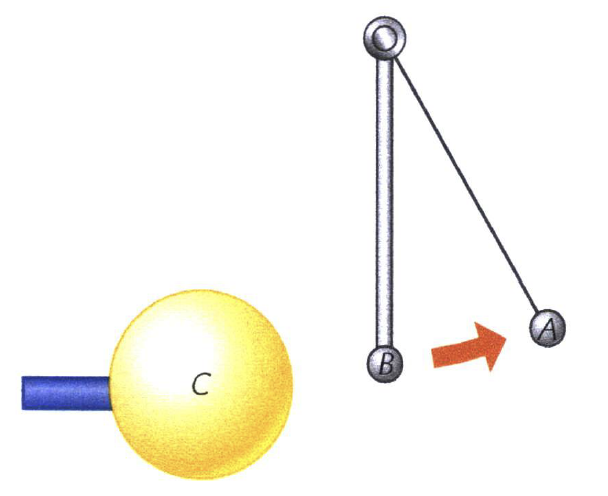
\includegraphics[width=.35\textwidth]{./img/ch1_electrostatics_lq_2024-06-18-17-27-20.png}\par}
    \begin{parts}
        \part 當一個帶電導體$C$靠近小球$B$,兩者沒有接 觸,小球$A$便會擺起,如圖。
        \begin{subparts}
            \subpart 試解釋小球 $A$ 為甚麼會擺起。\zzh{2}
            \subpart 拿開導體$C$後,試描述小球$A$ 的運動。\zzh{1}
        \end{subparts}
        \part 現在,導體$C$與小球$B$觸碰,小球$A$ 比原來 擺起更大幅度。
        \begin{subparts}
            \subpart 假設小球的質量各為$m$。問懸起小球$A$ 的尼龍繩,其張力為多少? \zzh{3}
            \subpart 試描述小球$A$ 在導體$C$拿開後的運動。\zzh{1}
        \end{subparts}
    \end{parts}
    \dlines{1}\clearpage
}{
    % \src{Active Physics p67 q11}
    \par{\par\centering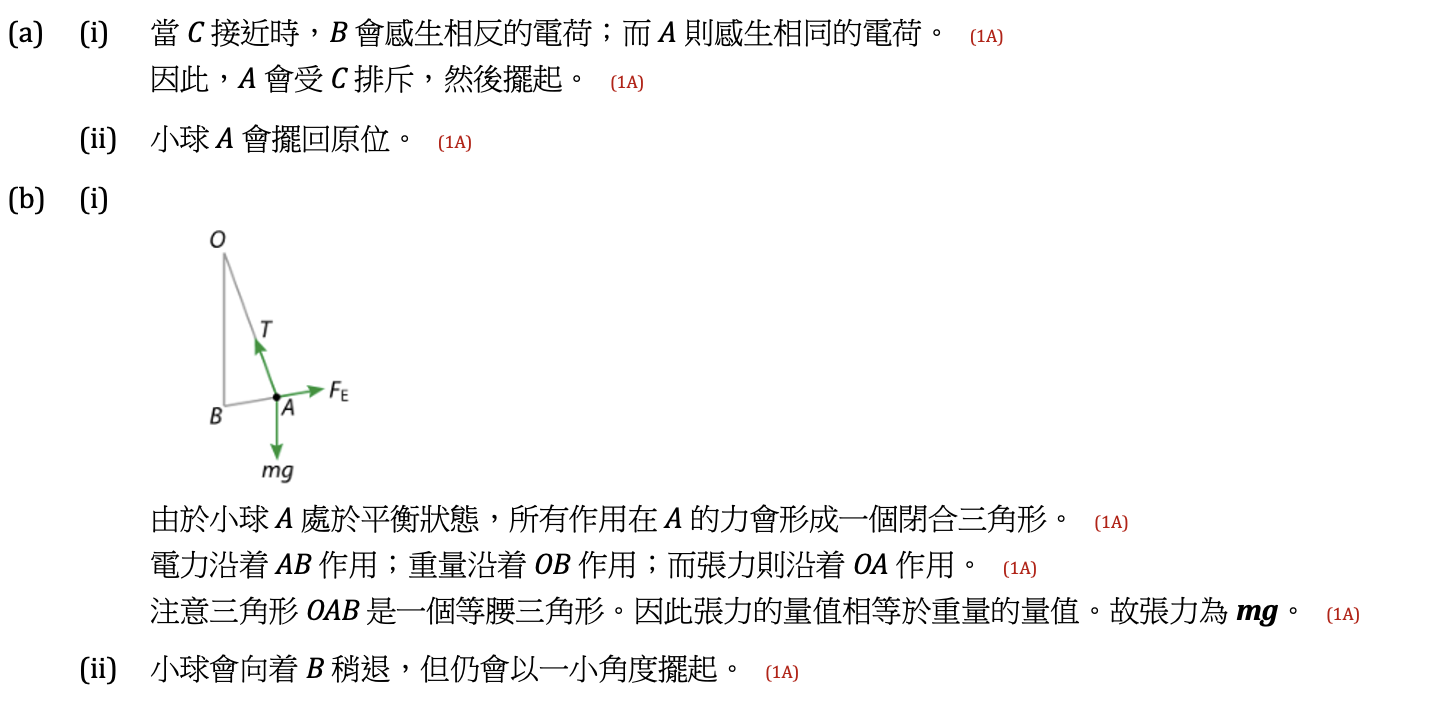
\includegraphics[width=\textwidth]{./img/ch1_electrostatics_lq_2024-06-18-17-31-06.png}\par}
}